\vspace{0.4cm}
\begin{mdframed}[backgroundcolor=black] 
\begin{center}
\vspace{0.6cm}
\parbox[t]{0.85\textwidth}{
\center
\texttt{\textcolor{white}{\fontsize{10}{7}\selectfont{\textbf{You can piece together information from the sparse and noisy data and reconstruct the image of something that by definition is impossible to see.}}}}
\vspace{1.5cm}
}
\makebox[\textwidth][c]{
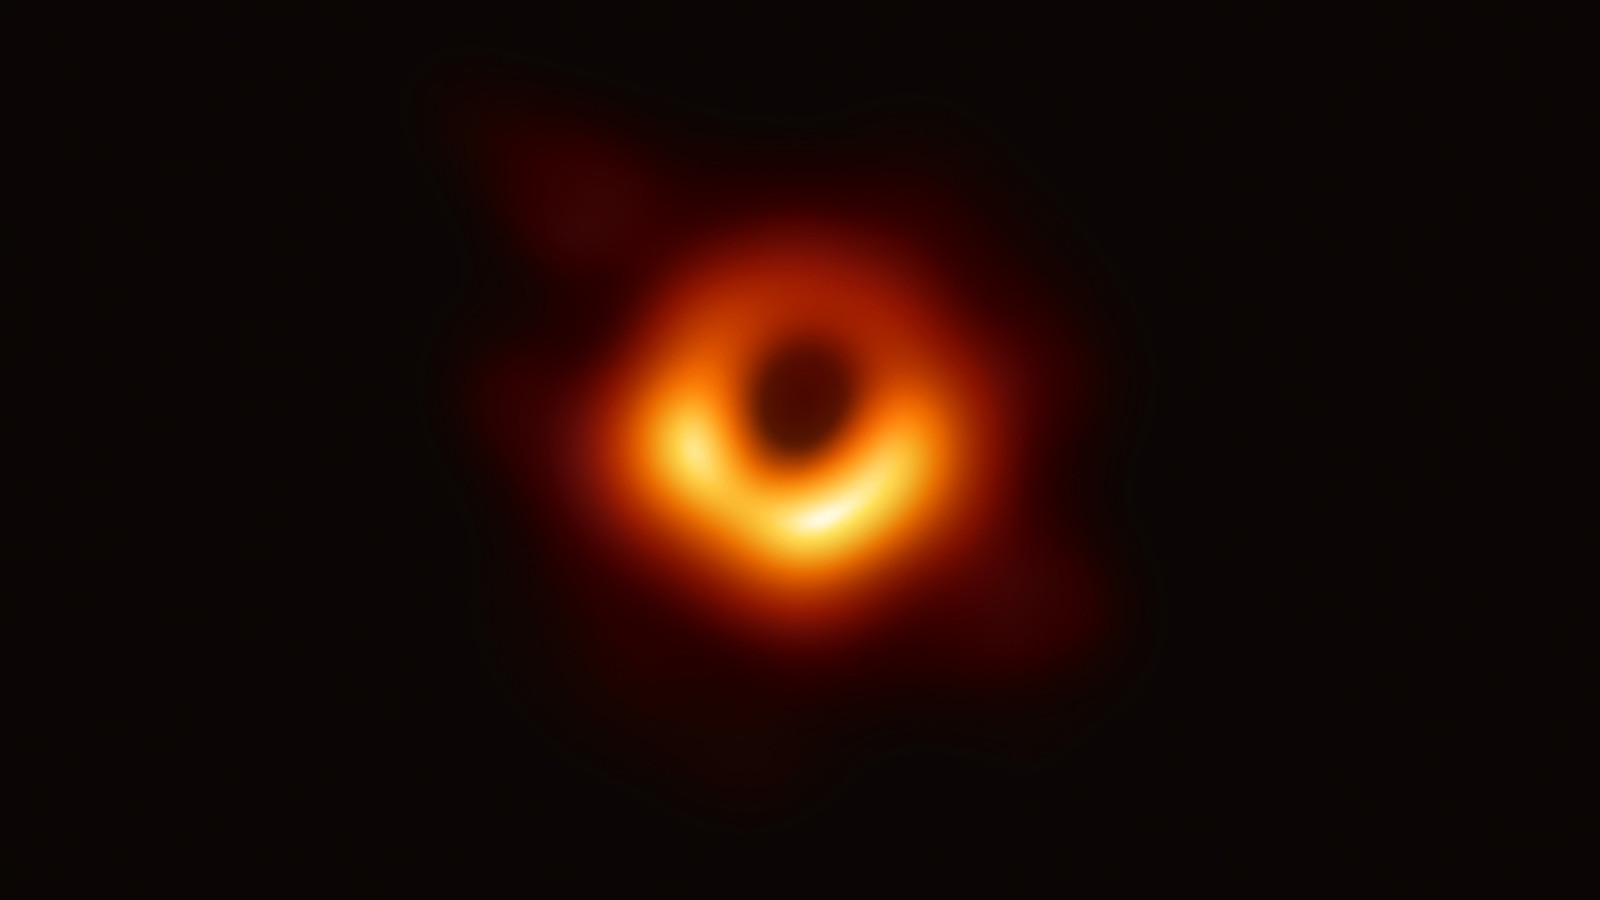
\includegraphics[height=8cm, width=\textwidth]{05-conclusions/figs_and_tables/blackhole.jpg}
}
\parbox[t]{192pt}{
\vspace{-1.5cm}
\texttt{\textcolor{white}{\fontsize{5}{4}\selectfont{\textbf{The first-ever image of a black hole in the center of the galaxy M87, reconstructed by the Event Horizon Telescope project in 2019, using the data from telescopes around the earth.}}}}}
\vspace{1.5cm}
\end{center}
\end{mdframed}
